\documentclass[11pt,a4paper]{article}

\usepackage[margin=1in]{geometry}
\usepackage{amsmath}
\usepackage{graphicx}
\usepackage[T1]{fontenc}
\usepackage[utf8]{inputenc}
\usepackage{lmodern}
\usepackage[hidelinks]{hyperref}

\graphicspath{{docs/images/algorithms/}{../images/algorithms/}}

\title{Derived Signals in EvalData\\A Small Algorithm Note}
\author{EvalData Repository Example}
\date{April 2026}

\begin{document}

\maketitle

\section{Purpose}

This note explains the current derived-signal operations exposed in the EvalData analysis workspace. The examples are reproducible because they use the built-in spectral and input-output demo datasets.

Derived signals create new columns from existing columns. They do not overwrite the original loaded dataset; they extend the working dataframe used inside one analysis workspace session.

\section{Operation Set}

The current UI exposes five derived-signal operations:

\begin{itemize}
    \item \textbf{delta}: first difference,
    \item \textbf{ratio}: source divided by a second column,
    \item \textbf{rolling\_mean}: moving average written as a derived column,
    \item \textbf{derivative}: discrete rate of change with respect to a reference column or index,
    \item \textbf{normalized}: z-score normalization, or mean-centering when the standard deviation is zero.
\end{itemize}

\section{Difference-Based Signals}

\subsection{Delta}

For a sampled signal $x[n]$, the delta operation is

\[
\Delta x[n] = x[n] - x[n-1].
\]

It highlights local changes between adjacent samples.

\subsection{Derivative}

When a reference axis $t[n]$ is available, EvalData computes a discrete derivative as

\[
\frac{dx}{dt}[n] \approx \frac{x[n] - x[n-1]}{t[n] - t[n-1]}.
\]

If no external reference column is selected, the row index plays the role of the reference axis.

\begin{figure}[ht]
    \centering
    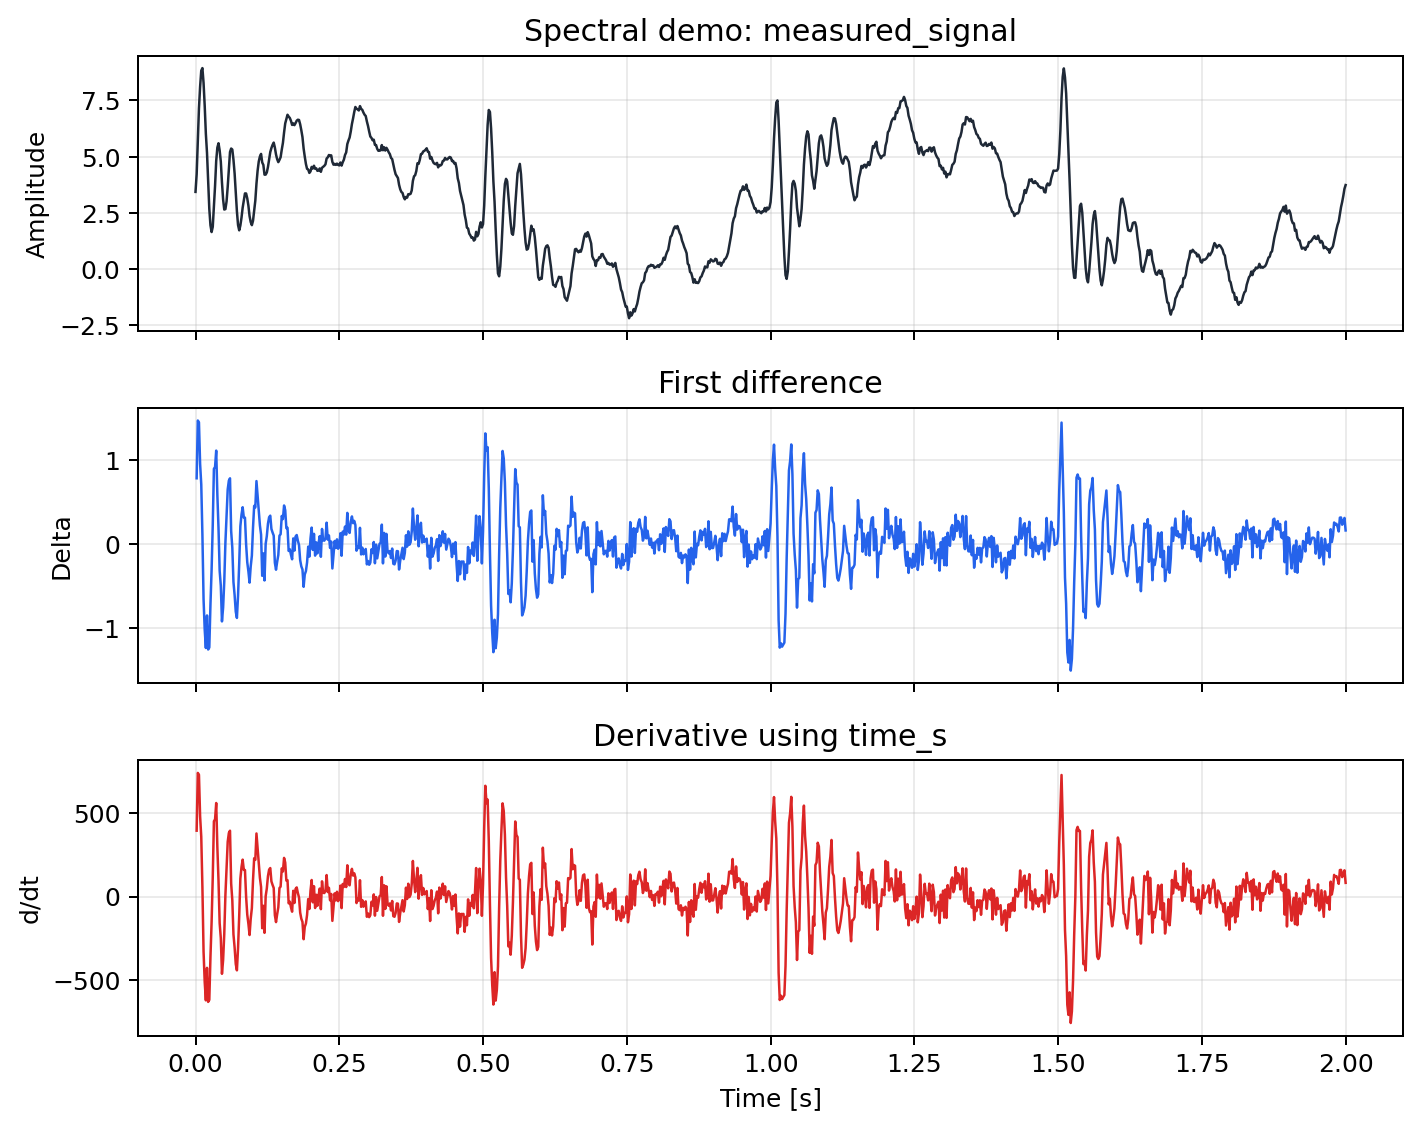
\includegraphics[width=0.92\linewidth]{derived_delta_derivative_example.png}
    \caption{Reproducible derived-signal example on the built-in spectral demo. The first difference emphasizes sample-to-sample jumps, while the derivative scales the same idea by the time axis.}
\end{figure}

\section{Ratio and Rolling Mean}

\subsection{Ratio}

For source $x[n]$ and denominator $z[n]$, the ratio is

\[
r[n] = \frac{x[n]}{z[n]}.
\]

In the current implementation, zero denominators are replaced by \texttt{NaN} before division. This avoids a hard divide-by-zero failure, but it also means the resulting column may contain missing values wherever the denominator vanishes.

\subsection{Rolling Mean}

For an odd window width $W = 2m + 1$, the rolling mean is

\[
y[n] = \frac{1}{W} \sum_{k=-m}^{m} x[n+k].
\]

This is mathematically the same local average used in the filtering note, but here it is exposed as a derived signal operation rather than as a dedicated filter action.

\section{Normalization}

EvalData's normalized operation uses

\[
z[n] = \frac{x[n] - \mu_x}{\sigma_x},
\]

where $\mu_x$ is the sample mean and $\sigma_x$ is the sample standard deviation with $ddof=1$.

If $\sigma_x = 0$ or is undefined, the implementation falls back to mean-centering:

\[
z[n] = x[n] - \mu_x.
\]

\begin{figure}[ht]
    \centering
    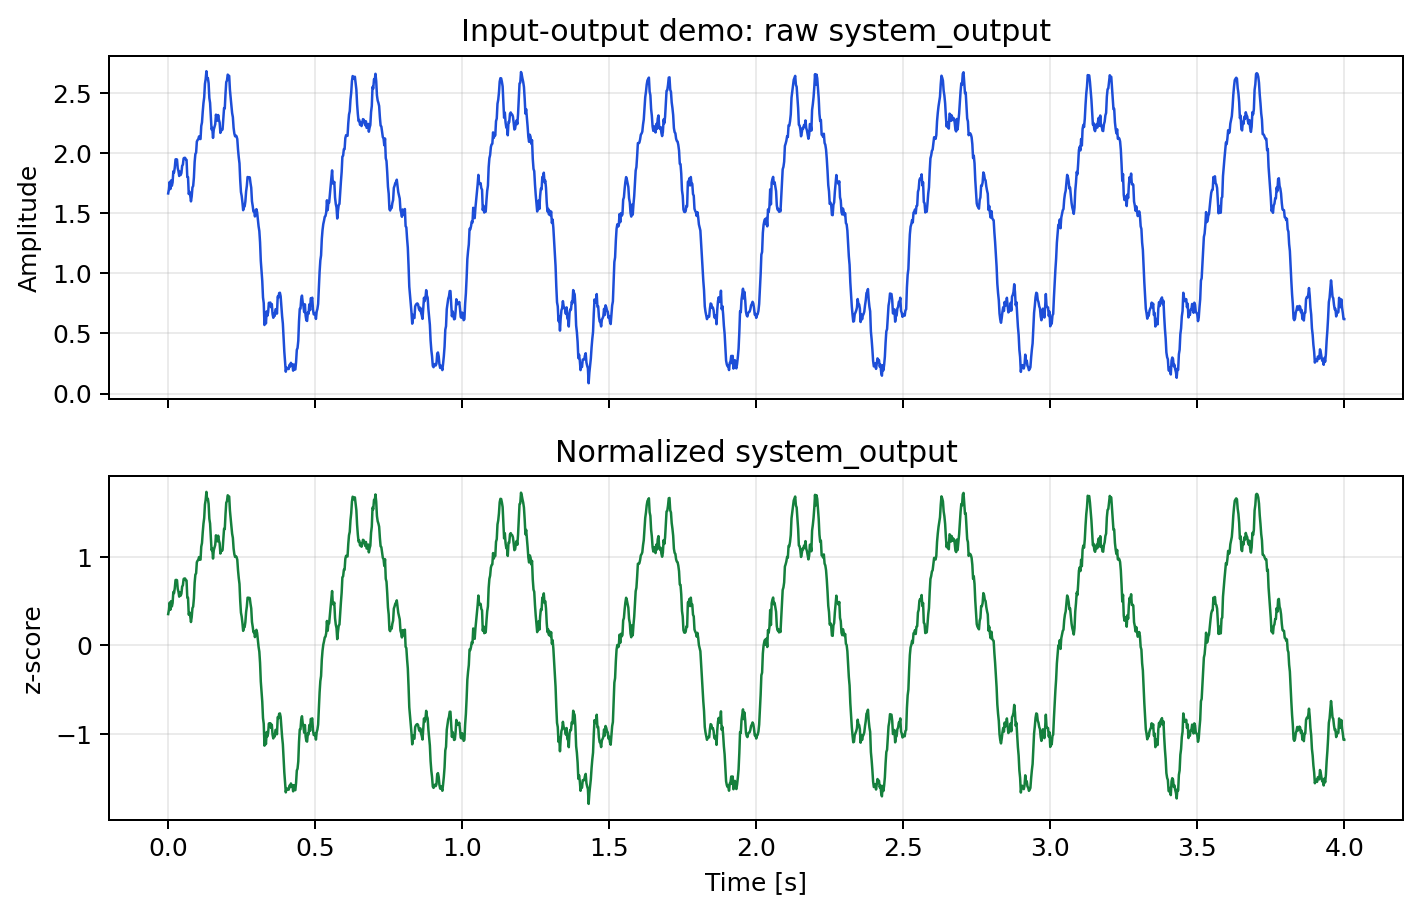
\includegraphics[width=0.92\linewidth]{derived_normalized_example.png}
    \caption{Normalization on the built-in input-output demo. The lower plot shows the same \texttt{system\_output} channel after z-score scaling.}
\end{figure}

\section{What the Demo Cases Show}

The spectral demo is useful for delta and derivative because it contains impacts, ringing, drift, and smooth periodic content in the same deterministic record. The input-output demo is useful for normalization because the output channel has a nonzero offset and a different scale from the other signals.

\section{Practical Interpretation Limits}

\begin{itemize}
    \item Delta and derivative amplify noise and abrupt discontinuities.
    \item Derivative results are only meaningful if the reference axis is interpreted correctly.
    \item Ratios become unstable when the denominator is near zero, even if exact zeros are suppressed.
    \item Normalized signals lose their original engineering units.
    \item Rolling means smooth data, but they also blur short transients.
\end{itemize}

\section{Conclusion}

Derived signals are lightweight transformations that make specific behaviors easier to see: change, relative scaling, local trend, rate of change, or scale-free variation. They are mathematically simple, but they change the meaning of the signal enough that the documentation should state the formulas explicitly.

\end{document}